\section{基于DCM的双足(人形)机器人行走轨迹生成与控制}
    该章主要根据文献\cite{englsbergerThreedimensionalBipedalWalking2013}的内容进行重新整理和复现,下面介绍相关内容。
    \subsection{DCM基本动力学方程的推导与几种特征点的定义}
        \subsubsection{DCM(运动发散量)的定义}
            DCM(Divergent Component of Motion),将其定义为相对机器人质心的偏移点,其定义式如下:
            \begin{equation}
                \boldsymbol{\xi }=\boldsymbol{x}+b\boldsymbol{\dot{x}}
                \label{equ2-1}
            \end{equation}

            式\eqref{equ2-1}变形后可得到质心的动力学方程:
            \begin{equation}
                \boldsymbol{\dot{x}}=-\frac{1}{b}\left( \boldsymbol{x}-\boldsymbol{\xi } \right) 
                \label{equ2-2}
            \end{equation}
            其中,当$b>0$时可得到稳定的一阶动力学方程。

            将式\eqref{equ2-1}求一阶导并代入$m\boldsymbol{\ddot{x}}=\boldsymbol{F}$可得DCM动力学方程:
            \begin{equation}
                \boldsymbol{\dot{\xi}}=-\frac{1}{b}\boldsymbol{x}+\frac{1}{b}\boldsymbol{\xi }+\frac{b}{m}\boldsymbol{F} 
                \label{equ2-3}
            \end{equation}
        \subsubsection{eCMP的定义}
            eCMP(Enhanced Centroidal Moment Pivot Point),与式\eqref{equ1-1}中的外力定义形式类似,此处
            将接触作用外力与eCMP定义联系,其关系定义如下,其中$s>0$且为常数:
            \begin{equation}
                \boldsymbol{F}_{ext}=s\left( \boldsymbol{x}-\boldsymbol{r}_{ecmp} \right) 
                \label{equ2-4}
            \end{equation}

            再将上式加上重力所求得合力的代入式\eqref{equ2-3}可得下式\eqref{equ2-5a},再选择
            常数$s=\frac{m}{b^2}$可化简得下式\eqref{equ2-5b}:
            \begin{subequations}
                \begin{align}
                    \boldsymbol{\dot{\xi}} &= \left( \frac{bs}{m}-\frac{1}{b} \right) \boldsymbol{x}+\frac{1}{b}\boldsymbol{\xi }-\frac{bs}{m}\boldsymbol{r}_{ecmp}+b\boldsymbol{g}
                    \label{equ2-5a}\\
                    \boldsymbol{\dot{\xi}} &= \frac{1}{b}\boldsymbol{\xi }-\frac{1}{b}\boldsymbol{r}_{ecmp}+b\boldsymbol{g}
                    \label{equ2-5b}
                \end{align}
            \end{subequations}
        \subsubsection{VRP的定义}
            引入VRP(Virtual Repellent Point)来进一步化简上式\eqref{equ2-5b},定义VRP如下:
            \begin{equation}
                \boldsymbol{r}_{vrp}=\boldsymbol{r}_{ecmp}+\left[ \begin{matrix}
                    0&		0&		b^2g\\
                \end{matrix} \right] ^T=\boldsymbol{r}_{ecmp}+\left[ \begin{matrix}
                    0&		0&		\varDelta z_{vrp}\\
                \end{matrix} \right] ^T
                \label{equ2-6}
            \end{equation}
            将其代入式\eqref{equ2-5b}可得最终形式的DCM动力学方程:
            \begin{equation}
                \boldsymbol{\dot{\xi}}=\frac{1}{b}\left( \boldsymbol{\xi }-\boldsymbol{r}_{vrp} \right) =\sqrt{\frac{g}{\varDelta z_{vrp}}}\left( \boldsymbol{\xi }-\boldsymbol{r}_{vrp} \right)
                \label{equ2-7}
            \end{equation}
            其中$b=\sqrt{\frac{\varDelta z_{vrp}}{g}}$将其代入式\eqref{equ2-4}则可得所有合外力:
            \begin{subequations}
                \begin{align}
                    \boldsymbol{F}&=\frac{m}{b^2}\left( \boldsymbol{x}-\boldsymbol{r}_{vrp} \right) 
                    \label{equ2-8a}\\
                    \boldsymbol{F}&=\frac{mg}{\varDelta z_{vrp}}\left( \boldsymbol{x}-\boldsymbol{r}_{vrp} \right) 
                    \label{equ2-8b}
                \end{align}               
            \end{subequations}
            最后的质心CoM动力学方程为:
            \begin{equation}
                \boldsymbol{\dot{x}}=-\sqrt{\frac{g}{\varDelta z_{vrp}}}\left( \boldsymbol{x}-\boldsymbol{\xi } \right) 
                \label{equ2-9}
            \end{equation}
            所有特征点的示意图如下所示:
            \begin{figure}[h] 
                \centering
                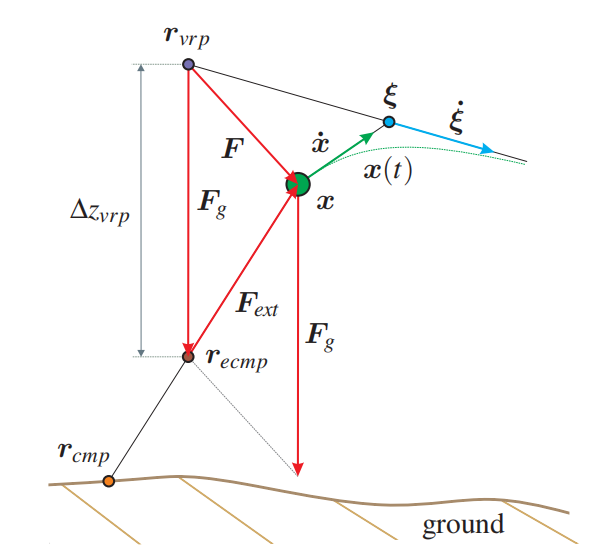
\includegraphics[scale=0.4]{2021-08-17-10-53-23.png}
                \caption{所定义特征点的示意图} \label{fig2-1}
            \end{figure}
            \FloatBarrier
    \subsection{几种不同支撑类型下的DCM、CoM轨迹生成}
        \subsubsection{单点支撑SS(Single Support)情形}
            假设机器人的足为单点或支撑点位于脚掌中心,机器人角动量变化为0,且随着双脚切换时支点的移动是
            瞬时的(没有双脚同时受力的情形),则此时令脚支撑点$\boldsymbol{r}_{f,i}$、压力中心$\boldsymbol{r}_{cop}$(Center of Pressure)、
            中心动量支点$\boldsymbol{r}_{cmp}$(Centroidal Moment Pivot Point)以及$\boldsymbol{r}_{ecmp}$重合,这几种点
            的作用示意图如下图\ref{fig2-2a}所示,重合情况见下图\ref{fig2-2b},该方法使得CoP为常量,接触外力总通过质心。
            \begin{figure}[h] 
                \centering
                \subfloat[CoP、CMP、eCMP等点的定义]{
                    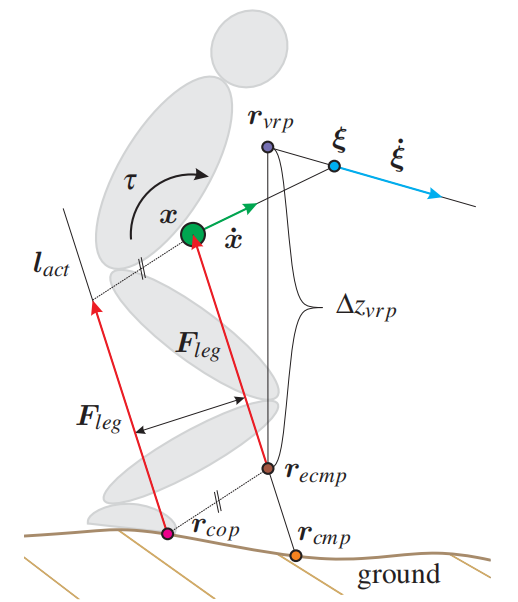
\includegraphics[scale=0.35]{2021-08-17-11-55-16.png}
                    \label{fig2-2a}
                }
                \vspace{5pt} %两图的竖直间隔
                \subfloat[单点支撑时各点重合]{
                    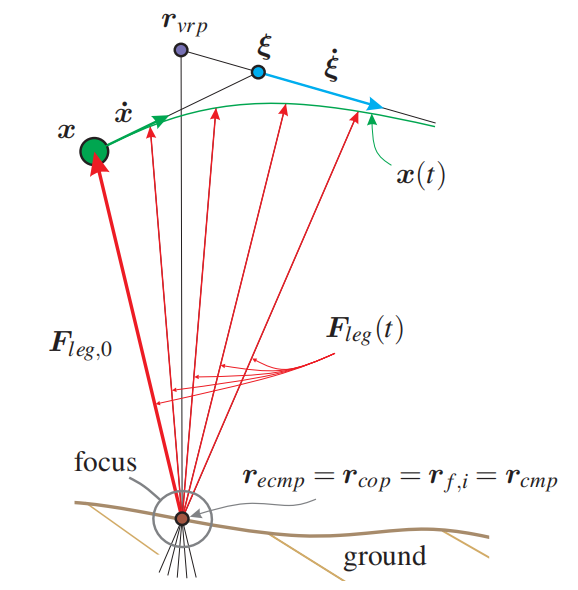
\includegraphics[scale=0.35]{2021-08-17-11-57-17.png}
                    \label{fig2-2b}
                }
                \caption{各点定义及单点支撑的示意图} \label{fig2-2}
            \end{figure}
            \FloatBarrier

            首先设定N个落脚点$\boldsymbol{r}_f,i$,限定单点支撑时VRP的位置为该支撑点竖直偏移$\varDelta z_{vrp}$(因为此时CoP与eCMP重合)
            即$z_{vrp,d,i}=z_{f,i}+\varDelta z_{vrp}$,由此VRP的位置在第$i$个支撑点作用时为常量,求解方程\ref{equ2-7}可得:
            \begin{equation}
                \boldsymbol{\xi }\left( t \right) =\boldsymbol{r}_{vrp}+e^{\sqrt{\frac{g}{\varDelta z_{vrp}}}t}\left( \boldsymbol{\xi }\left( 0 \right) -\boldsymbol{r}_{vrp} \right)
                \label{equ2-10}
            \end{equation}
            设定每一段的单个支撑点作用时间为$t_{step,i}$,则上述$t\in \left[ 0,t_{step,i} \right]$。设定最后机器人在第N个支撑点停下,
            下标$d$表示目标值(desired),$eos$表示end of support,此时$\boldsymbol{\xi}_{d,eos,N-1}=\boldsymbol{r}_{vrp,d,N}$,
            可以通过向后迭代推算出每一段支撑运动的DCM起始值$\boldsymbol{\xi}_{d,ini,N-1}$与终止值$\boldsymbol{\xi}_{d,eos,N-1}$,
            根据式\ref{equ2-10}建立迭代式如下:
            \begin{equation}
                \boldsymbol{\xi }_{d,eos,i-1}=\boldsymbol{\xi }_{d,ini,i}=\boldsymbol{r}_{vrp,d,i}+e^{-\sqrt{\frac{g}{\varDelta z_{vrp}}}t_{step,i}}\left( \boldsymbol{\xi }_{d,eos,i}-\boldsymbol{r}_{vrp,d,i} \right) 
                \label{equ2-11}
            \end{equation}
            再将迭代结果代回式\ref{equ2-10}并求导可得到DCM在每段的动力学解,即得到DCM轨迹:
            \begin{subequations}
                \begin{align}
                    \boldsymbol{\xi }_{d,i}\left( t \right) &=\boldsymbol{r}_{vrp,d,i}+e^{\sqrt{\frac{g}{\varDelta z_{vrp}}}\left( t-t_{step,i} \right)}\left( \boldsymbol{\xi }_{d,eos,i}-\boldsymbol{r}_{vrp,d,i} \right) 
                    \label{equ2-12a}\\
                    \boldsymbol{\dot{\xi}}_{d,i}\left( t \right) &=\sqrt{\frac{g}{\varDelta z_{vrp}}}e^{\sqrt{\frac{g}{\varDelta z_{vrp}}}\left( t-t_{step,i} \right)}\left( \boldsymbol{\xi }_{d,eos,i}-\boldsymbol{r}_{vrp,d,i} \right) 
                    \label{equ2-12b}
                \end{align}
            \end{subequations}
            文献\cite{englsbergerThreedimensionalBipedalWalking2013}中的示意图如下图\ref{fig2-3}所示,规定好开始时CoM的位置$\boldsymbol{x}_0$以及
            VRP偏移eCMP的高度$\varDelta z_{vrp}$便可完成规划,可取$\varDelta z_{vrp}$为机器人单(双)腿直立站立静止时CoM与eCMP或支撑点的相对高度,使以上
            模型成立,到终点时CoM速度为零,DCM、CoM与VRP重合(DCM先与VRP重合然后COM跟随一段时间才与DCM重合)。由于初始的DCM位置由脚步点规划后的反向迭代结果确定,因此初始点$\boldsymbol{x}_0$的选择决定了
            初始CoM速度$\boldsymbol{\dot{x}}_0$。
            \begin{figure}[h] 
                \centering
                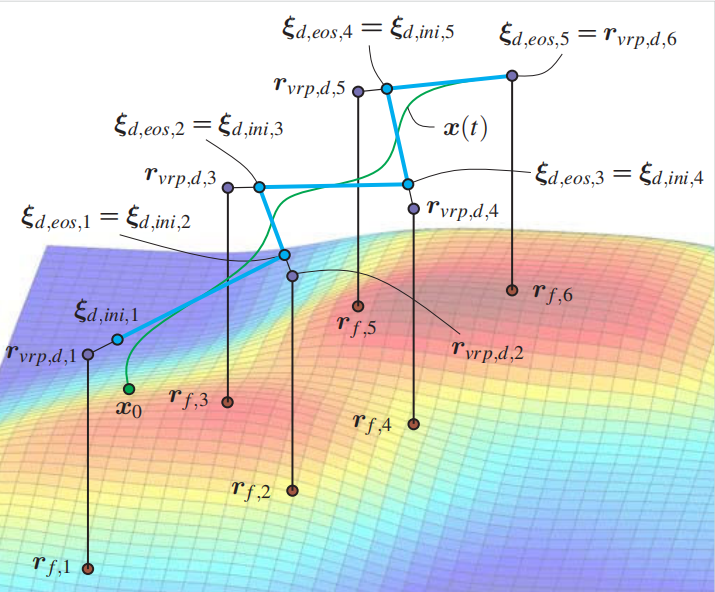
\includegraphics[scale=0.3]{2021-08-17-14-26-05.png}
                \caption{单点支撑DCM轨迹规划示意图} \label{fig2-3}
            \end{figure}
            \FloatBarrier

            利用python编写相关程序,预先给定6个落脚点,每段步利用4阶龙格库塔方法求解CoM的轨迹,当DCM到达终点之后一段的CoM轨迹则直接用修改Eular格式
            的单步迭代法求解,具体结果如下图\ref{fig2-4}所示,显示了各个点、每步的时间以及总时间等信息。
            \begin{figure}[h] 
                \centering
                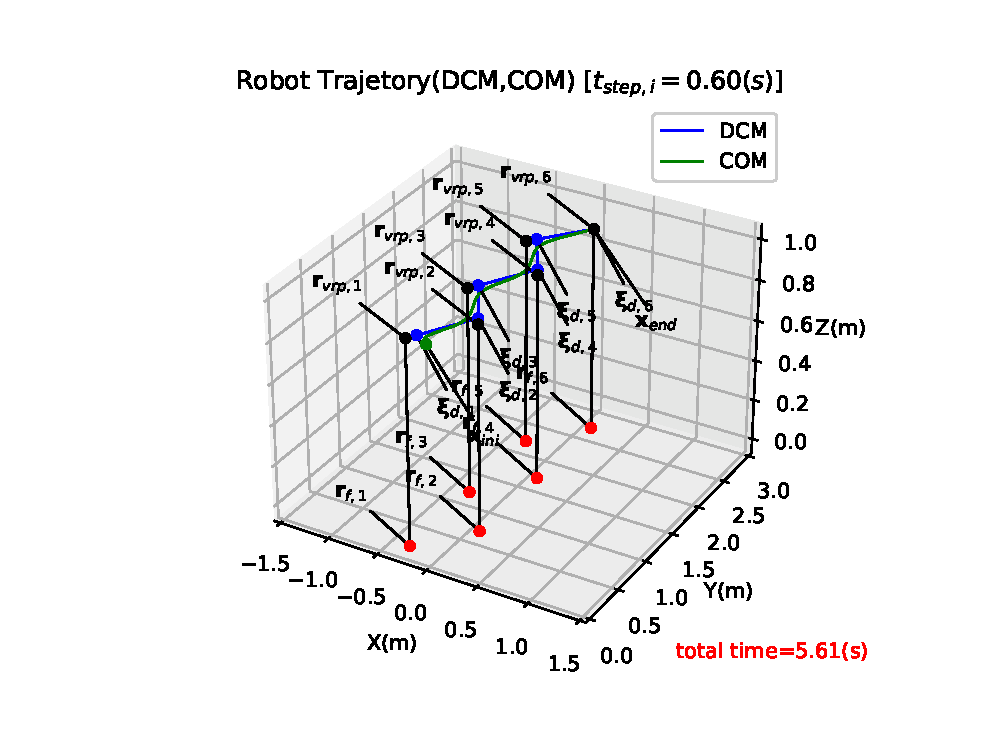
\includegraphics[scale=0.45]{DCM_SS.eps}
                \caption{复现单点支撑DCM轨迹规划图} \label{fig2-4}
            \end{figure}
            \FloatBarrier
        \subsubsection{连续双点支撑DS(Double Support)情形}
            由式\eqref{equ2-7}可知$\boldsymbol{r}_{vrp}$可由DCM表示:
            \begin{equation}
                \boldsymbol{r}_{vrp}=\boldsymbol{\xi }-\sqrt{\frac{\varDelta z_{vrp}}{g}}\boldsymbol{\dot{\xi}}
                \label{equ2-13}
            \end{equation}
            若DCM轨迹连续则VRP轨迹连续,并可进一步得到连续的外力,因此可在DCM的折点附近定义两个点用于插值,且DCM处于此两点之间时机器人处于双足支撑状态,
            即两个单点支撑状态间的均匀过渡,支点CoP、eCMP随VRP的连续运动也连续变化。单步DCM折点附近双足支撑的起始点定义为$\boldsymbol{\xi}_{iniDS,i}$,
            终止点定义为$\boldsymbol{\xi}_{eoDS,i}$,单步时起点到折点的时间为$\varDelta t_{DS,ini}$,起点到折点的时间为$\varDelta t_{DS,end}$其过程
            示意图为图\ref{fig2-5},且两者及其对应速度可由如下公式计算:
            \begin{subequations}
                \begin{align}
                    \boldsymbol{\xi }_{iniDS,i}&=\boldsymbol{r}_{vrp,i-1}+e^{-\sqrt{\frac{g}{\varDelta z_{vrp}}}\varDelta t_{DS,ini}}\left( \boldsymbol{\xi }_{ini,i}-\boldsymbol{r}_{vrp,i-1} \right) 
                    \label{equ2-14a}\\
                    \boldsymbol{\xi }_{eoDS,i}&=\boldsymbol{r}_{vrp,i}+e^{\sqrt{\frac{g}{\varDelta z_{vrp}}}\varDelta t_{DS,end}}\left( \boldsymbol{\xi }_{ini,i}-\boldsymbol{r}_{vrp,i} \right) 
                    \label{equ2-14b}\\
                    \boldsymbol{\dot{\xi}}_{iniDS,i}&=\sqrt{\frac{g}{\varDelta z_{vrp}}}e^{-\sqrt{\frac{g}{\varDelta z_{vrp}}}\varDelta t_{DS,ini}}\left( \boldsymbol{\xi }_{ini,i}-\boldsymbol{r}_{vrp,i-1} \right) 
                    \label{equ2-14c}\\
                    \boldsymbol{\dot{\xi}}_{eoDS,i}&=\sqrt{\frac{g}{\varDelta z_{vrp}}}e^{\sqrt{\frac{g}{\varDelta z_{vrp}}}\varDelta t_{DS,end}}\left( \boldsymbol{\xi }_{ini,i}-\boldsymbol{r}_{vrp,i} \right) 
                    \label{equ2-14d}
                \end{align}
            \end{subequations}
            \begin{figure}[h] 
                \centering
                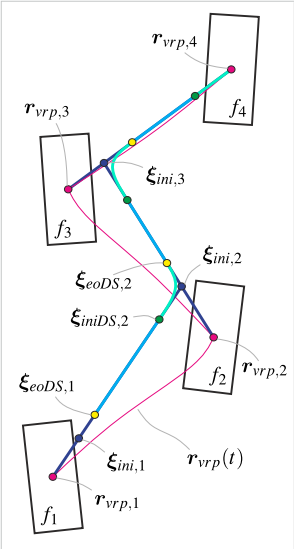
\includegraphics[scale=0.6]{2021-08-21-23-07-46.png}
                \caption{双点支撑DCM轨迹规划示意图} \label{fig2-5}
            \end{figure}
            \FloatBarrier

            双足支撑的起点$\boldsymbol{\xi}_{iniDS,i}$与终止点$\boldsymbol{\xi}_{eoDS,i}$之间的轨迹点可用三次多项式插值产生,给定位置与速度的4个边界条件,按以下公式计算:
            \begin{subequations}
                \begin{align}
                    \boldsymbol{P} = \left[
                    \begin{matrix}
                        2/{T_s}^3&		1/{T_s}^2&		-2/{T_s}^3&		1/{T_s}^2\\
                        -3/{T_s}^2&		-2/T_s&		3/{T_s}^2&		-1/T_s\\
                        0&		1&		0&		0\\
                        1&		0&		0&		0\\
                    \end{matrix} \right] \left[ 
                    \begin{array}{c}
                        \xi _{ini}^{T}\\
                        \dot{\xi}_{ini}^{T}\\
                        \xi _{end}^{T}\\
                        \dot{\xi}_{end}^{T}\\
                    \end{array} \right] 
                    \label{equ2-15a}\\
                    \left[ \begin{array}{c}
                        \boldsymbol{\xi }^T\left( t \right)\\
                        \boldsymbol{\dot{\xi}}^T\left( t \right)\\
                    \end{array} \right] =\left[ \begin{matrix}
                        t^3&		t^2&		t&		1\\
                        3t^2&		2t&		1&		0\\
                    \end{matrix} \right] \boldsymbol{P}
                    \label{equ2-15b}
                \end{align}
            \end{subequations}

            设定好相关参数后,用Python编写双足支撑下的CoM、DCM规划程序,自定义六个落脚点以及初始CoM位置并进行规划,规划结果与相关参数如下图\ref{fig2-6}所示,
            其中$\varDelta t_{DS,ini,i}=\alpha\varDelta t_{DS,i}$、$\varDelta t_{DS,end,i}=(1-\alpha)\varDelta t_{DS,i}$。
            \begin{figure}[ht] 
                \centering
                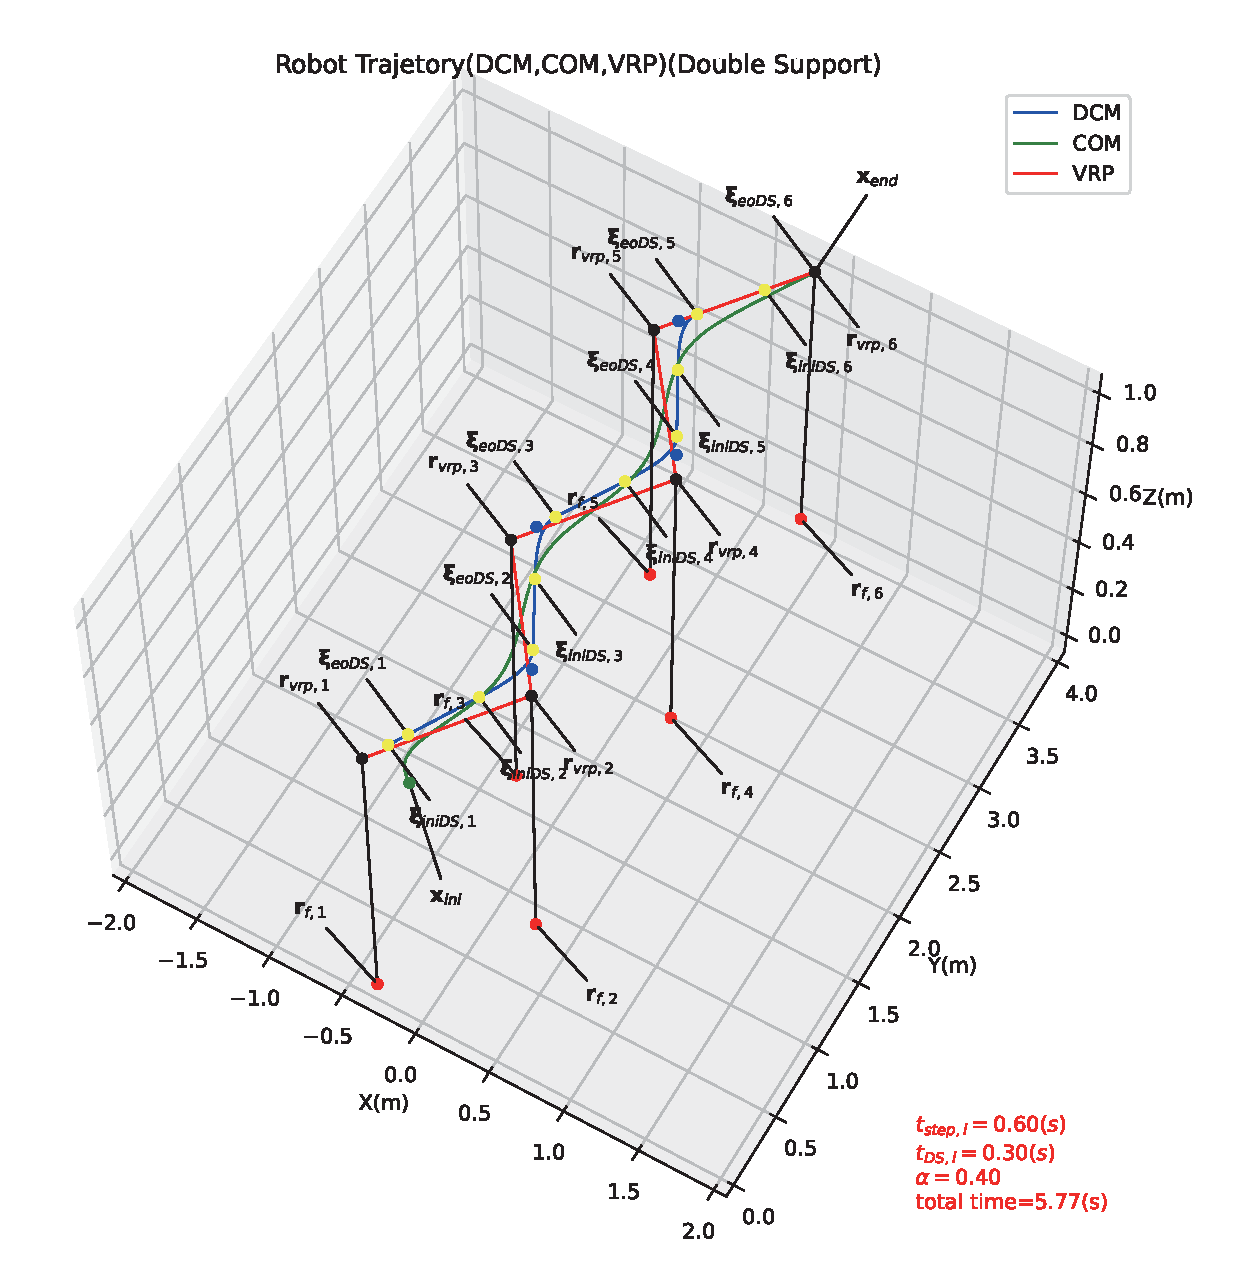
\includegraphics[scale=0.5]{DCM_DS.eps}
                \caption{复现双点支撑DCM轨迹规划图} \label{fig2-6}
            \end{figure}
            \FloatBarrier
        \subsubsection{连续足跟-足尖运动支撑切换HT(Heel to Toe)情形}
            上一小节中讨论的双足支撑机器人的脚固定在地面,为使机器人在双足支撑时的运动尽可能避开奇异构型并与人更为类似,现考虑加入足跟到足尖与足尖到足跟的连续支撑点切换。
            该动作可扩大机器人单步运动的行程与范围,但在足尖与脚跟切换时其支撑多边形范围会变小。采用该动作时的轨迹示意图如下图\ref{fig2-7}所示,将单步时间$t_{step,i}$
            拆分为足跟到足尖支撑时间$\varDelta t_{HT}=\alpha_{HT}t_{step,i}$与足尖到足跟支撑时间$\varDelta t_{TH}=(1-\alpha_{HT})t_{step,i}$并可采用2.2.1单点支撑后向递推
            的方法算出各个DCM节点$\boldsymbol{\xi}_{ini,HT,i}$与$\boldsymbol{\xi}_{ini,TH,i}$,在每个脚跟DCM节点$\boldsymbol{\xi}_{ini,HT,i}$附近用上一小节式\eqref{equ2-14a}到\eqref{equ2-14d}的方法计算出双足
            支撑的DCM起始点与、终止点及其速度。
            \begin{figure}[h] 
                \centering
                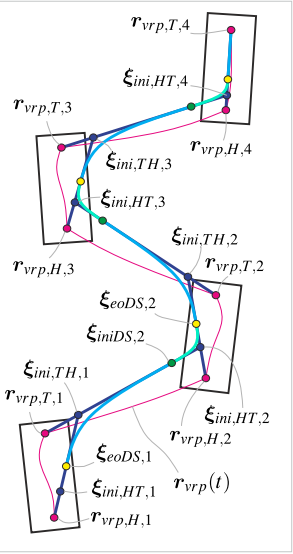
\includegraphics[scale=0.6]{2021-08-24-14-28-10.png}
                \caption{足跟-足尖支撑DCM轨迹规划示意图} \label{fig2-7}
            \end{figure}
            \FloatBarrier
            对该方法的复现结果与相关参数如下图\ref{fig2-8}所示,其中开始时$\boldsymbol{\xi}_{ini,HT,1}$到$\boldsymbol{\xi}_{eoDS,1}$的DCM轨迹与末尾$\boldsymbol{\xi}_{eoDS,end}$到$\boldsymbol{r}_{vrp,end}$的DCM轨迹
            由式\eqref{equ2-15a}和\eqref{equ2-15b}计算得到,并利用式\eqref{equ2-13}推导出VRP轨迹,但最后一段利用插值所计算出的VRP轨迹超出了所在足跟和足尖的范围。
            \begin{figure}[h] 
                \centering
                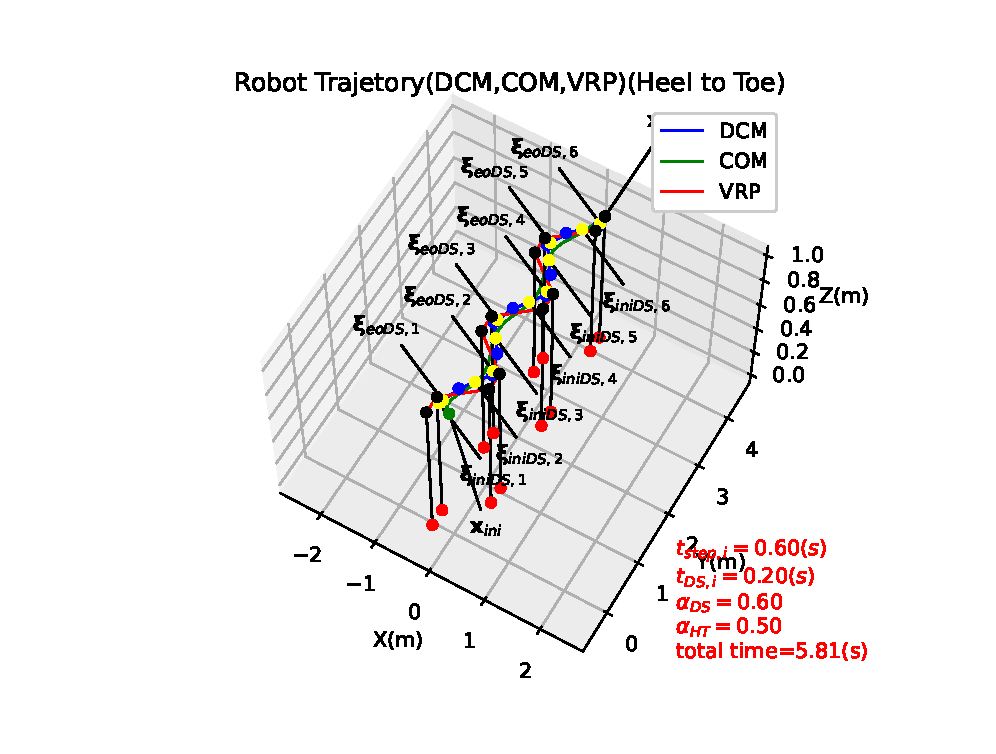
\includegraphics[scale=0.5]{DCM_HT.eps}
                \caption{复现足跟-足尖支撑DCM轨迹规划图} \label{fig2-8}
            \end{figure}
            \FloatBarrier
    \subsection{DCM运动轨迹跟随控制}
        由于DCM动力学方程的解发散,需要对上述DCM规划的运动轨迹做跟随控制,引入一阶闭环动力学控制对DCM轨迹做位置跟随:
        \begin{equation}
            \underset{\boldsymbol{\dot{e}}_{\xi}}{\underbrace{\boldsymbol{\dot{\xi}}-\boldsymbol{\dot{\xi}}_d}}=-k_{\xi}\underset{\boldsymbol{e}_{\xi}}{\underbrace{\left( \boldsymbol{\xi }-\boldsymbol{\xi }_d \right) }}
            \label{equ2-16}
        \end{equation}
        当$k_{\xi}>0$时误差收敛到0,DCM速度、位置均收敛,由式\eqref{equ2-13}可知此时VRP位置也收敛,但常VRP位置受扰动发生了改变(之前在假设机器人进入单足支撑状态时VRP为固定常量),
        VRP在闭环动力学下的方程如下式\eqref{equ2-17a}所示,代入式$\boldsymbol{\dot{\xi}}_d=\sqrt{\frac{g}{\varDelta z_{vrp}}}\left( \boldsymbol{\xi }_d-\boldsymbol{r}_{vrp,d,1} \right)$可得目标VRP位置
        为常量时实际偏移后的VRP位置如下式\eqref{equ2-17b}所示。
        \begin{subequations}
            \begin{align}
                \boldsymbol{r}_{vrp}&=\boldsymbol{\xi }+k_{\xi}\sqrt{\frac{\varDelta z_{vrp}}{g}}\left( \boldsymbol{\xi }-\boldsymbol{\xi }_d \right) -\sqrt{\frac{\varDelta z_{vrp}}{g}}\boldsymbol{\dot{\xi}}_d
                \label{equ2-17a}\\
                \boldsymbol{r}_{vrp}&=\boldsymbol{r}_{vrp,d,1}+\left( 1+k_{\xi}\sqrt{\frac{\varDelta z_{vrp}}{g}} \right) \left( \boldsymbol{\xi }-\boldsymbol{\xi }_d \right) 
                \label{equ2-17b}
            \end{align}
        \end{subequations}

        CoM动力学方程的收敛性没有变化,但其方程需代入式\eqref{equ2-16}进行修改,与DCM闭环动力学方程一起写成矩阵形式如下:
        \begin{equation}
            \left[ \begin{array}{c}
                \boldsymbol{\dot{x}}\\
                \boldsymbol{\dot{\xi}}\\
            \end{array} \right] =\left[ \begin{matrix}
                -\sqrt{\frac{g}{\varDelta z_{vrp}}}\boldsymbol{I}&		\sqrt{\frac{g}{\varDelta z_{vrp}}}\boldsymbol{I}\\
                0&		-k_{\xi}\boldsymbol{I}\\
            \end{matrix} \right] \left[ \begin{array}{c}
                \boldsymbol{x}\\
                \boldsymbol{\xi }\\
            \end{array} \right] +\left[ \begin{matrix}
                0&		0\\
                k_{\xi}\boldsymbol{I}&		\boldsymbol{I}\\
            \end{matrix} \right] \left[ \begin{array}{c}
                \boldsymbol{\xi }_d\\
                \boldsymbol{\dot{\xi}}_d\\
            \end{array} \right]
            \label{equ2-18}
        \end{equation}
        其中系统矩阵的特征值在$k_{\xi}>0$时均大于0,此时系统稳定,CoM、DCM均可收敛到理想值。机器人所受合外力表达式为:
        \begin{equation}
            \boldsymbol{F}_c=\frac{m}{b^2}\left( \boldsymbol{x}-\boldsymbol{\xi }-k_{\xi}b\left( \boldsymbol{\xi }-\boldsymbol{\xi }_d \right) +b\boldsymbol{\dot{\xi}}_d \right) 
            \label{equ2-19}
        \end{equation}
    \subsection{DCM运动控制鲁棒性分析}
        根据上一小节的DCM跟随控制分别对CoM估计误差、常外力扰动、未知力迟滞、质量估计误差几个情况做鲁棒性分析。现假设传感器
        和滤波器估计的实际CoM位置表示为$\hat{\boldsymbol{x}}$,由估计的CoM位置与速度计算出的DCM位置为$\hat{\boldsymbol{\xi}}$,测量估计
        质量为$\hat{m}$,由于机器人整体的运动需通过外界与机器人的接触力来驱动,据式\eqref{equ2-19}由观测估计值计算得到的合外力为:
        \begin{equation}
            \boldsymbol{F}_c=\frac{\hat{m}}{b^2}\left( \boldsymbol{\hat{x}}-\boldsymbol{\hat{\xi}}-k_{\xi}b\left( \boldsymbol{\hat{\xi}}-\boldsymbol{\xi }_d \right) +b\boldsymbol{\dot{\xi}}_d \right) 
            \label{equ2-20}
        \end{equation}
        \subsubsection{对CoM估计误差的鲁棒性分析}
            设估计偏差为$\varDelta \boldsymbol{x}$,则CoM位置与速度估计值如下:
            \begin{subequations}
                \begin{align}
                    \boldsymbol{\hat{x}}&=\boldsymbol{x}+\varDelta \boldsymbol{x} 
                    \label{equ2-21a}\\
                    \boldsymbol{\dot{\hat{x}}}&=\boldsymbol{\dot{x}}+\varDelta \boldsymbol{\dot{x}}
                    \label{equ2-21b}
                \end{align}
            \end{subequations}
            将上式代入DCM定义式\eqref{equ2-1}可得到估计的DCM状态:
            \begin{equation}
                \boldsymbol{\hat{\xi}}=\boldsymbol{\xi }+\varDelta \boldsymbol{x}+b\varDelta \boldsymbol{\dot{x}}
                \label{equ2-22}
            \end{equation}

            由式\eqref{equ2-20}计算的合外力代入DCM动力学方程式\eqref{equ2-3},再结合CoM动力学方程可得如下闭环动力学方程:
            \begin{equation}
                \left[ \begin{array}{c}
                    \boldsymbol{\dot{x}}\\
                    \boldsymbol{\dot{\xi}}\\
                \end{array} \right] =\left[ \begin{matrix}
                    -\frac{1}{b}\boldsymbol{I}&		\frac{1}{b}\boldsymbol{I}\\
                    0&		-k_{\xi}\boldsymbol{I}\\
                \end{matrix} \right] \left[ \begin{array}{c}
                    \boldsymbol{x}\\
                    \boldsymbol{\xi }\\
                \end{array} \right] +\left[ \begin{matrix}
                    0&		0\\
                    k_{\xi}\boldsymbol{I}&		\boldsymbol{I}\\
                \end{matrix} \right] \left[ \begin{array}{c}
                    \boldsymbol{\xi }_d\\
                    \boldsymbol{\dot{\xi}}_d\\
                \end{array} \right] +\left[ \begin{matrix}
                    0&		0\\
                    -k_{\xi}\boldsymbol{I}&		-\left( k_{\xi}b+1 \right) \boldsymbol{I}\\
                \end{matrix} \right] \left[ \begin{array}{c}
                    \varDelta \boldsymbol{\dot{x}}\\
                    \varDelta \boldsymbol{x}\\
                \end{array} \right] 
                \label{equ2-23}
            \end{equation}

            若CoM估计误差$\varDelta \boldsymbol{x}$为常数,则DCM误差动力学方程及其解变为如下:
            \begin{subequations}
                \begin{align}
                    \boldsymbol{\dot{\xi}}&=-k_{\xi}\boldsymbol{\xi }+k_{\xi}\boldsymbol{\xi }_d+\boldsymbol{\dot{\xi}}_d-k_{\xi}\varDelta \boldsymbol{x},\left( \varDelta \boldsymbol{\dot{x}}=0 \right)
                    \label{equ2-24a}\\
                    \boldsymbol{\dot{\xi}}-\boldsymbol{\dot{\xi}}_d&=-k_{\xi}\left( \boldsymbol{\xi }-\boldsymbol{\xi }_d \right) -k_{\xi}\varDelta \boldsymbol{x}
                    \label{equ2-24b}\\
                    \boldsymbol{e}_{\xi}\left( t \right) &=-\varDelta \boldsymbol{x}+e^{-k_{\xi}t}\left( \boldsymbol{e}_{\xi ,0}+\varDelta \boldsymbol{x} \right)
                    \label{equ2-24c}
                \end{align}
            \end{subequations}
            因此此时存在静态误差$e_{\xi,stat}=-\varDelta \boldsymbol{x}$。
        \subsubsection{未知常外力扰动时的鲁棒性分析}
            假设机器人受到未知常外力$\varDelta \boldsymbol{F}$,机器人实际所受合外力为$\boldsymbol{F}=\boldsymbol{F_c}+\varDelta \boldsymbol{F}$。将其代入
            式\eqref{equ2-19}并与式\eqref{equ2-3}联立可得以下闭环动力学方程:
            \begin{equation}
                \left[ \begin{array}{c}
                    \boldsymbol{\dot{x}}\\
                    \boldsymbol{\dot{\xi}}\\
                \end{array} \right] =\left[ \begin{matrix}
                    -\frac{1}{b}\boldsymbol{I}&		\frac{1}{b}\boldsymbol{I}\\
                    0&		-k_{\xi}\boldsymbol{I}\\
                \end{matrix} \right] \left[ \begin{array}{c}
                    \boldsymbol{x}\\
                    \boldsymbol{\xi }\\
                \end{array} \right] +\left[ \begin{matrix}
                    0&		0\\
                    k_{\xi}\boldsymbol{I}&		\boldsymbol{I}\\
                \end{matrix} \right] \left[ \begin{array}{c}
                    \boldsymbol{\xi }_d\\
                    \boldsymbol{\dot{\xi}}_d\\
                \end{array} \right] +\left[ \begin{array}{c}
                    0\\
                    \frac{b}{m}\boldsymbol{I}\\
                \end{array} \right] \varDelta \boldsymbol{F} 
                \label{equ2-25}
            \end{equation}
            动力学方程在$k_{\xi}>0$及$b>0$时稳定,与上一小节同理,可得到DCM误差:
            \begin{equation}
                \boldsymbol{e}_{\xi}\left( t \right) =\frac{b\varDelta \boldsymbol{F}}{mk_{\xi}}+e^{-k_{\xi}t}\left( \boldsymbol{e}_{\xi ,0}-\frac{b\varDelta \boldsymbol{F}}{mk_{\xi}} \right) 
                \label{equ2-26}
            \end{equation}
            静态误差$e_{\xi,stat}=\frac{b\varDelta \boldsymbol{F}}{mk_{\xi}}$,类似于线弹性效应,其中刚度为$\frac{mk_{\xi}}{b}$。
        \subsubsection{未知力迟滞情况的鲁棒性分析}
            对于实际的机器人硬件,无法瞬时产生所需的力,作用力会有所延迟,此处将该延迟效应表示如下:
            \begin{equation}
                \boldsymbol{\dot{F}}=-k_f\left( \boldsymbol{F}-\boldsymbol{F}_c \right)
                \label{equ2-27}
            \end{equation}
            其中$\boldsymbol{F}$为实际作用力,$\boldsymbol{F}_c$为所需的目标作用力,$k_f>0$。

            由式\eqref{equ2-27}、式\eqref{equ2-3}与式\eqref{equ2-19}可得出闭环动力学方程为:
            \begin{equation}
                \left[ \begin{array}{c}
                    \boldsymbol{\dot{x}}\\
                    \boldsymbol{\dot{\xi}}\\
                    \boldsymbol{\dot{F}}\\
                \end{array} \right] =\left[ \begin{matrix}
                    -\frac{1}{b}\boldsymbol{I}&		\frac{1}{b}\boldsymbol{I}&		0\\
                    -\frac{1}{b}\boldsymbol{I}&		\frac{1}{b}\boldsymbol{I}&		\frac{b}{m}\boldsymbol{I}\\
                    \frac{mk_f}{b^2}\boldsymbol{I}&		-\frac{mk_f\left( 1+k_{\xi}b \right)}{b^2}\boldsymbol{I}&		-k_f\boldsymbol{I}\\
                \end{matrix} \right] \left[ \begin{array}{c}
                    \boldsymbol{x}\\
                    \boldsymbol{\xi }\\
                    \boldsymbol{F}\\
                \end{array} \right] +\left[ \begin{matrix}
                    0&		0\\
                    0&		0\\
                    \frac{mk_fk_{\xi}}{b}\boldsymbol{I}&		\frac{mk_f}{b}\boldsymbol{I}\\
                \end{matrix} \right] \left[ \begin{array}{c}
                    \boldsymbol{\xi }_d\\
                    \boldsymbol{\dot{\xi}}_d\\
                \end{array} \right]
                \label{equ2-28}
            \end{equation}
            可利用MATLAB计算该动力学矩阵的特征值多项式,代码如下:
            \begin{lstlisting}
syms b k_xi m positive real
syms k_f real
syms lambda
syms I matrix real

dynm = [-1/b*I              1/b*I                0*I;
        -1/b*I              1/b*I               b/m*I;
    m*k_f/(b^2)*I  -m*k_f*(1+k_xi*b)/(b^2)*I    -k_f*I] %dynamics matrix

eigpoly = charpoly(dynm,lambda); %calculate characteristic polynomial
eigpoly = subs(eigpoly, I, 1)
root = solve(eigpoly, lambda, 'MaxDegree',3) %calculate the eigenvalues in explict form
            \end{lstlisting}

            计算结果如下:
            \begin{subequations}
                \begin{equation}
                    \textrm{eigpoly}=k_f \,\lambda^2 +\lambda^3 +\frac{\lambda \,{\left(k_f +b\,k_f \,k_{\xi } \right)}}{b}+\frac{k_f \,k_{\xi } }{b} 
                    \label{equ2-29a}\\
                \end{equation}
                \begin{equation}    
                    \begin{array}{c}
                       \textrm{root}=\left(\begin{array}{c}
                        \sigma_1 -\frac{\sigma_2 }{\sigma_1 }-\frac{k_f }{3}\\
                        \frac{\sigma_2 }{2\,\sigma_1 }-\frac{k_f }{3}-\frac{\sigma_1 }{2}-\frac{\sqrt{3}\,{\left(\frac{\sigma_2 }{\sigma_1 }+\sigma_1 \right)}\,\mathrm{i}}{2}\\
                        \frac{\sigma_2 }{2\,\sigma_1 }-\frac{k_f }{3}-\frac{\sigma_1 }{2}+\frac{\sqrt{3}\,{\left(\frac{\sigma_2 }{\sigma_1 }+\sigma_1 \right)}\,\mathrm{i}}{2}
                        \end{array}\right)\\
                        \mathrm{}\\
                        \textrm{where}\\
                        \mathrm{}\\
                        \;\;\sigma_1 ={{\left(\sqrt{{\sigma_2 }^3 +{{\left(\frac{{k_f }^3 }{27}-\frac{k_f \,{\left(k_f +b\,k_f \,k_{\xi } \right)}}{6\,b}+\frac{k_f \,k_{\xi } }{2\,b}\right)}}^2 }-\frac{{k_f }^3 }{27}+\frac{k_f \,{\left(k_f +b\,k_f \,k_{\xi } \right)}}{6\,b}-\frac{k_f \,k_{\xi } }{2\,b}\right)}}^{1/3} \\
                        \mathrm{}\\
                        \;\;\sigma_2 =\frac{k_f +b\,k_f \,k_{\xi } }{3\,b}-\frac{{k_f }^2 }{9}
                        \end{array}
                        \label{equ2-29b}
                \end{equation}
            \end{subequations}
    







